\scanpage{4}
\uline{Formules utiles}
\[
1728\Delta=c_4^3-c_6^2
\]
\[
j=\frac{c_4^3}{\Delta}=1728+c_6^2/\Delta
\]
\[
c_4\in H^0(\unsure{\overline{\Pi}|\overline{M}},\omega^4)\quad
c_6=H^0(\unsure{\overline{\Pi}|\overline{M}},\omega^6)\quad
\Delta=H^0(\unsure{\overline{\Pi}|\overline{M}},\omega^{12}
\]
\margin{car $\ne 2,3$.}
\[
\begin{aligned}
c_4=0&\Longleftrightarrow 6\text{ auto}\Longleftrightarrow j=0\\
c_6=0&\Longleftrightarrow 4\text{ auto}\Longleftrightarrow j=1728
\end{aligned}
\]
\[
h\in H^0(\unsure{\overline{\Pi}|\overline{M}},\omega^{\otimes\deleted{\unsure{12}}\inserted{p-1}})
\]
\[
\deg\omega=1/24
\]
\figure{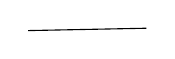
\begin{tikzpicture}\draw (0,0)--(1.5,.03);\end{tikzpicture}}
\[
\begin{aligned}
E=G_m/q^{\mathbb Z},\ \frac{du}{u}\quad\to\quad
c_4&=\left(\frac{du}{u}\right)^{\otimes4}\left(1+240\sum\sigma_3(n)q^n\right)\qquad(=E_4)\quad(Q)\\
c_6&=\left(\frac{du}{u}\right)^{\otimes6}\left(1\deleted{\unsure{+}}\inserted{-}504\sum\sigma_5(n)q^n\right)\qquad(=E_6)\quad(R)
\end{aligned}
\]
\figure{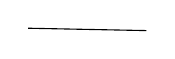
\begin{tikzpicture}\draw (0,0)--(1.5,-.03);\end{tikzpicture}}

Question : $h=\left(\dfrac{du}{u}\right)^{\otimes p-1}$ ? à l'$\infty$ --

\figure{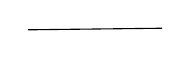
\begin{tikzpicture}\draw (0,0)--(1.7,.02);\end{tikzpicture}}
\[
y^2=x(x-1)(x-\lambda)\quad\longmapsto\quad j=2^8\frac{(1-\lambda(1-\lambda))^3}{(\lambda(1-\lambda))^2}
\]
\margin{[$\unsure{p^{\mathrm{ts}}}$ ordre 2 marqués]
\diagram{$\boxed{\begin{array}{l}
\lambda\\1-\lambda\\\lambda^{-1}\\1-\lambda^{-1}\\(1-\lambda)^{-1}\\\unsure{-}(1-\lambda^{-1})^{-1}
\end{array}}$}}
\figure{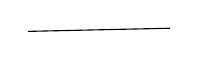
\begin{tikzpicture}\draw (0,0)--(1.8,.04);\end{tikzpicture}}
\uline{Hasse} : $(-1)^n\sum\binom{n}{i}^2\lambda^i$

ou $n=\dfrac{p-1}{2}$

\diagram{$\begin{array}{c@{\quad}cccc@{\quad}l}
p\equiv&1&5&7&11&(12)\\
\lambda=& &0&1728&\begin{array}{c}0\\1728\end{array}&\text{et }\dfrac{p-\unsure{\bullet}}{12}\text{ autres --}
\end{array}$}
\figure{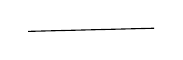
\begin{tikzpicture}\draw (0,0)--(1.6,.04);\end{tikzpicture}}
\margin{3}
